\documentclass[../../D1.tex]{subfiles}

\begin{document}
In this section we present the design considerations for the software that will be developed in conjunction with this research project.

\subsection{Functional Requirements}
\subsubsection{Inference Agent}
The inference agent will function as a dedicated inference benchmarking and reporting tool. It will listen for queued models, run the inference benchmarks with the model and send the results to a queue dedicated to the sender of the model.

\begin{table}[h]
    \begin{tabular}{@{}l|p{10cm}|l@{}}
    \toprule
    Code   & Description                                             & Importance \\ \midrule
    IA.FR1 & Subscribe to inference queue                            & High       \\
    IA.FR2 & Download ONNX model from queue                          & High       \\
    IA.FR3 & Run OpenVINO benchmark with model                       & High       \\
    IA.FR4 & Parse benchmark metrics                                 & High       \\
    IA.FR5 & Pulish metrics to queue corresponding to training agent & HIgh       \\ \bottomrule
    \end{tabular}
\end{table}

\subsubsection{Training Agent}
The training agent will be responsible for applying the compression algorthm to the model and, once compression is complete, it will send the model to an inference queue.
\begin{table}[h]
    \begin{tabular}{@{}l|p{10cm}|l@{}}
    \toprule
    Code   & Description                                                        & Importance \\ \midrule
    TA.FR1 & Apply compression a to given model based on a set of parameters    & High       \\
    TA.FR2 & Enqueue ONNX model to inference queue with an agent identifier     & High       \\
    TA.FR3 & Await the return of the benchmarking metrics via a dedicated queue & High       \\
    TA.FR4 & Send metrics to Weights and Baises for recording                   & High       \\ \bottomrule
    \end{tabular}
    \end{table}

\subsubsection{Optimiser Interface}
The optimiser interface is a fairly simple program that is purely concerned with constructing tweaked OpenVINO scheduler definitions based on concise sets of parameters, its purpose is to abstract away many parameters that we do not want to change run to run during experiments.
\begin{table}[h]
    \begin{tabular}{@{}l|p{10cm}|l@{}}
    \toprule
    Code   & Description                                                                                & Importance \\ \midrule
    OI.FR1 & Provide an interface for pruning parameters to be defined                                  & High       \\
    OI.FR2 & Construct an OpenVINO schedule based on some predefined defaults and the passed parameters & High       \\
    OI.FR3 & Produce a .yaml file defining the schedule                                                 & Medium     \\
    OI.FR4 & Log the .yaml schedule for future reuse                                                    & Low        \\ \bottomrule
    \end{tabular}
\end{table}


\subsection{Non-functional Requirements}
The following non-functional requirements apply to all 3 aspecst of the system.

\begin{table}[H]
    \begin{tabular}{l|p{10cm}|l}
    \hline
    Code & Description                                                                                                 & Importance \\ \hline
    NFR1 & Queue implementation should not be a bottleneck by itself                                                   & high       \\
    NFR2 & The system should be robust to the failure of a training agent                                              & medium     \\
    NFR3 & The system should not introduce any changes to the model other than those enacted by Distiller and OpenVINO & high       \\
    NFR4 & All benchmark metrics should have redundant storage                                                         & low        \\ \hline
    \end{tabular}
    \end{table}

\subsection{Optimisation and Benchmarking suite}\label{sec:ERdiagram}
%This section will display a high level design on the benchmarking and optimisation suite.

Figure~\ref{fig:benchcycle} shows an entity relationship diagram to depict the benchmark and optimisation suite, either a hand crafted initial set of paramaters are provided to a \emph{Training Agent} or they could be randomly initialised at the start of the optimisation cycle.
The training agent will use the optimiser interface each time new compression parameters are passed to it, this will construct the appropriate scheduler that the training agent will utilise.
This diagram also applies for the first set of experimental benchmarks (without an optimiser), in this case the \emph{Training Agent} will only train once with the specified compression parameters, and the cycle would terminate when the metrics are sent to Weights and Biases.

\begin{figure}[H]
    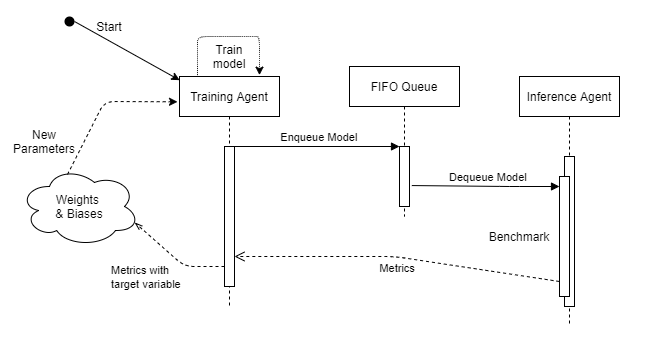
\includegraphics[width=1\textwidth]{dfd.png}
    \caption{Parameter optimisation ER diagram}
    \label{fig:benchcycle}
\end{figure}

Using this system we could theoretically benefit from adding new \emph{Training Agents} to the pool of agents until the consumers \emph{Inference Agent} are unable to clear the queue.
We intend to utilise at least two GPU, and one CPU \emph{Training Agents}, with a single \emph{Inference Agent} using the NCS


\end{document}